\chapter{Background}
\label{ch:background}

\section{Anomaly detection}
\index{anomaly detection}
\newglossaryentry{anomaly}{
    name=anomaly,
    plural=anomalies,
    description={patterns in data that do not conform to a well defined notion 
                 of normal behavior}
}
Anomaly detection is the process of detecting patterns in a given data set that 
do not conform to an established normal behavior \cite{CHANDOLA07}.

The importance of anomaly detection is due to the fact that anomalies in data
translate to significant (and often critical) actionable information in a wide 
variety of application domains \cite{CHANDOLA07}.

\subsection{What are anomalies?}
\index{anomaly}
\Gls{anomaly} are patterns in data that do not conform to a well defined notion 
of normal behavior. Figure~\ref{fig:2d-anomalies} illustrates anomalies in a 
simple 2-dimensional data set. The data has two normal regions, $N_{1}$ and 
$N_{2}$, since most observations lie in these two regions. Points that are 
sufficiently far away from the regions, such as points $o_{1}$ and $o_{2}$, and 
points in region $O_{3}$, are anomalies.

\begin{figure}[H]
\centering
\ifpdf
	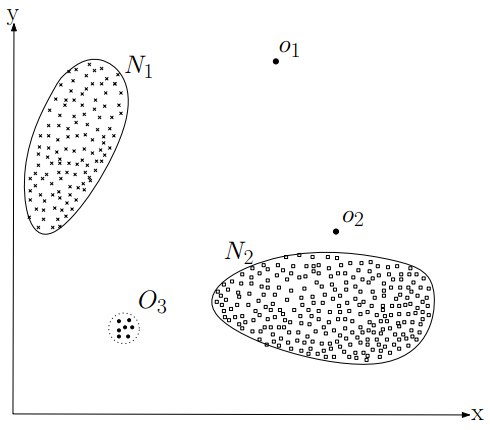
\includegraphics[width=0.5\textwidth]{2d-anomalies.png}
\else
	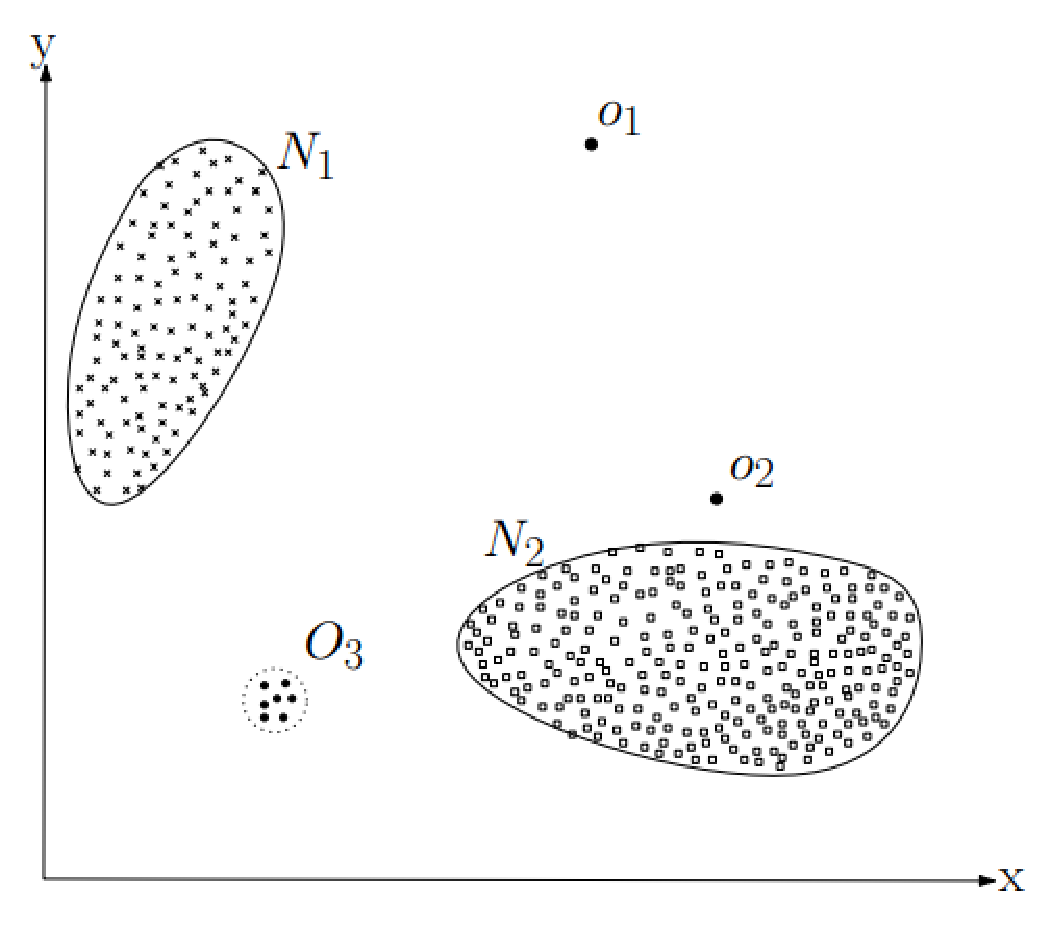
\includegraphics[width=0.5\textwidth]{2d-anomalies.eps}
\fi
\caption{A simple example of anomalies in a 2-dimensional data set.}
\label{fig:2d-anomalies}
\end{figure}

\subsection{Challenges}
At an abstract level, an anomaly is defined as a pattern that does not conform 
to expected normal behavior. A straightforward anomaly detection approach, 
therefore, is to define a region representing normal behavior and declare any 
observation in the data which does not belong to this normal region as an 
anomaly. But several factors make this apparently simple approach very 
challenging:
\begin{itemize}
\item Defining a normal region which encompasses every possible normal behavior 
is very difficult. In addition, the boundary between normal and anomalous 
behaviour is often not precise. Thus an anomalous observation which lies close
to the boundary can actually be normal, and vice-versa.
\item When anomalies are the result of malicious actions, the malicious 
adversaries often adapt themselves to make the anomalous observations appear 
like normal, thereby making the task of defining normal behavior more difficult.
\item In many domains normal behavior keeps evolving and a current notion of
normal behavior might not be su±ciently representative in the future.
\item The exact notion of an anomaly is different for different application 
domains. For example, in the medical domain a small deviation from normal (for
example, fluctuations in body temperature) might be an anomaly, while similar 
deviation in the stock market domain (for example, fluctuations in the value of 
a stock) might be considered as normal. Thus applying a technique developed in 
one domain to another is not straightforward.
\item Availability of labeled data for training/validation of models used by 
anomaly detection techniques is usually a major issue.
\item Often the data contains noise which tends to be similar to the actual 
anomalies and hence is di±cult to distinguish and remove.
\end{itemize}

Due to the above challenges, the anomaly detection problem, in its most general
form, is not easy to solve. In fact, most of the existing anomaly detection 
techniques solve a specific formulation of the problem. The formulation is 
induced by various factors such as nature of the data, availability of labeled 
data, type of anomalies to be detected, etc. Often, these factors are determined
by the application domain in which the anomalies need to be detected. 
Researchers have adopted concepts from diverse disciplines such as statistics, 
machine learning, data mining, information theory, spectral theory, and have 
applied them to specific problem formulations.

\section{Random projections}

\section{Distance metrics}
\index{distance,metric}
\newglossaryentry{distance}{
    name=distance,
    description={a quantitative description of how far apart three objects are}
}
\newglossaryentry{metric}{
    name=metric,
    description={a function describing how close or far away data points in some 
                 space are from each other}
}
\gls{distance} is a quantitative description of how far apart two objects are. 
Mathematically, a \gls{distance} or \gls{metric} is a function describing how 
close or far away data points in some space are from each other \cite{KHOA12}.

\subsection{Euclidean distance}
\subsection{Mahalanobis distance}
\subsection{Graph geodesic distance}

\section{Nearest Neighbour Algorithms}

% MATRICES
\section{Matrices}

\subsection{Eigenvectors}

\subsection{Laplacian Matrices}
\newglossaryentry{LaplacianMatrix}
{
    name={Laplacian Matrix},
    plural={Laplacian Matrices},
    description={a matrix representation of a graph}
}
A \gls{LaplacianMatrix} is a matrix representation of a graph. Given a simple 
graph $G$ with $n$ vertices, its Laplacian matrix $L := 
({\ell}_{i,j})_{n{\times}n}$ is defined as follows:
\begin{displaymath}
{\ell}_{i,j} := 
    \left\{
        \begin{array}{ll}
            deg(v_{i}) &    \quad \text{if $i = j$} \\
            -1 &            \quad \text{if $i \neq j$ and $v_{i}$ is adjacent to $v_{j}$} \\
            0 &             \quad \text{otherwise}
        \end{array}
    \right.
\end{displaymath}

The normalized Laplacian matrix is defined as:
\begin{displaymath}
{\ell}_{i,j} := 
    \left\{
        \begin{array}{ll}
            1 &                                             \quad \text{if $i = j$ and $deg(v_{i}) \neq 0$} \\
            \frac{-1}{\sqrt{deg(v_{i})deg(v_{j})}} & \quad  \text{if $i \neq j$ and $v_{i}$ is adjacent to $v_{j}$} \\
            0 &                                             \quad \text{otherwise}
        \end{array}
    \right.
\end{displaymath}

\subsection{Properties}
For a graph $G$ and its Laplacian Matrix $L$ with eigenvalues $\lambda_{0} <
\lambda_{1} < \ldots < \lambda_{n-1}$:

\begin{itemize}
\item $L$ is always positive-semidefinite ($\forall i, \lambda_{i} \geq 0; 
\lambda_{0} = 0$).
\item The number of times $0$ appears as an eigenvalue in the Laplacian Matrix 
is the number of connected components in the graph.
\item $\lambda_{0}$ is always $0$ because every Laplacian Matrix has an 
eigenvector of $\begin{bmatrix} 1 & 1 & \ldots & 1 \end{bmatrix}$ that, for each
row, adds the corresponding node's degree to a ``-1'' for each neighbour, 
thereby producing zero by definition.
\item The smallest non-zero eigenvalue of $L$ is called the spectral gap.
\item If we define an oriented incidence matrix $M$ with element $M_{ev}$ for 
edge $e$ (connecting vertex $i$ and $j$, with $i < j$) and vertex $v$ given by
\begin{displaymath}
M_{ev} := 
    \left\{
        \begin{array}{ll}
            1 &     \quad \text{if $v = i$} \\
            -1 &    \quad \text{if $v = j$} \\
            0 &     \quad \text{otherwise}
        \end{array}
    \right.
\end{displaymath}
then the Laplacian Matrix $L$ satisfies
\begin{displaymath}
L = M^{T}M
\end{displaymath}
\item The second smallest eigenvalue of $L$ is the algebraic connectivity of 
$G$.
\end{itemize}

\section{Commute Time}
\subsection{Anomaly Detection Using Commute Time}
